% Generated by Sphinx.
\def\sphinxdocclass{report}
\documentclass[letterpaper,10pt,english]{sphinxmanual}
\usepackage[utf8]{inputenc}
\DeclareUnicodeCharacter{00A0}{\nobreakspace}
\usepackage[T1]{fontenc}
\usepackage{babel}
\usepackage{times}
\usepackage[Bjarne]{fncychap}
\usepackage{longtable}
\usepackage{sphinx}


\title{py FITS IDI Documentation}
\date{May 11, 2011}
\release{0.1}
\author{Danny Price}
\newcommand{\sphinxlogo}{}
\renewcommand{\releasename}{Release}
\makeindex

\makeatletter
\def\PYG@reset{\let\PYG@it=\relax \let\PYG@bf=\relax%
    \let\PYG@ul=\relax \let\PYG@tc=\relax%
    \let\PYG@bc=\relax \let\PYG@ff=\relax}
\def\PYG@tok#1{\csname PYG@tok@#1\endcsname}
\def\PYG@toks#1+{\ifx\relax#1\empty\else%
    \PYG@tok{#1}\expandafter\PYG@toks\fi}
\def\PYG@do#1{\PYG@bc{\PYG@tc{\PYG@ul{%
    \PYG@it{\PYG@bf{\PYG@ff{#1}}}}}}}
\def\PYG#1#2{\PYG@reset\PYG@toks#1+\relax+\PYG@do{#2}}

\def\PYG@tok@gd{\def\PYG@tc##1{\textcolor[rgb]{0.63,0.00,0.00}{##1}}}
\def\PYG@tok@gu{\let\PYG@bf=\textbf\def\PYG@tc##1{\textcolor[rgb]{0.50,0.00,0.50}{##1}}}
\def\PYG@tok@gt{\def\PYG@tc##1{\textcolor[rgb]{0.00,0.25,0.82}{##1}}}
\def\PYG@tok@gs{\let\PYG@bf=\textbf}
\def\PYG@tok@gr{\def\PYG@tc##1{\textcolor[rgb]{1.00,0.00,0.00}{##1}}}
\def\PYG@tok@cm{\let\PYG@it=\textit\def\PYG@tc##1{\textcolor[rgb]{0.25,0.50,0.56}{##1}}}
\def\PYG@tok@vg{\def\PYG@tc##1{\textcolor[rgb]{0.73,0.38,0.84}{##1}}}
\def\PYG@tok@m{\def\PYG@tc##1{\textcolor[rgb]{0.13,0.50,0.31}{##1}}}
\def\PYG@tok@mh{\def\PYG@tc##1{\textcolor[rgb]{0.13,0.50,0.31}{##1}}}
\def\PYG@tok@cs{\def\PYG@tc##1{\textcolor[rgb]{0.25,0.50,0.56}{##1}}\def\PYG@bc##1{\colorbox[rgb]{1.00,0.94,0.94}{##1}}}
\def\PYG@tok@ge{\let\PYG@it=\textit}
\def\PYG@tok@vc{\def\PYG@tc##1{\textcolor[rgb]{0.73,0.38,0.84}{##1}}}
\def\PYG@tok@il{\def\PYG@tc##1{\textcolor[rgb]{0.13,0.50,0.31}{##1}}}
\def\PYG@tok@go{\def\PYG@tc##1{\textcolor[rgb]{0.19,0.19,0.19}{##1}}}
\def\PYG@tok@cp{\def\PYG@tc##1{\textcolor[rgb]{0.00,0.44,0.13}{##1}}}
\def\PYG@tok@gi{\def\PYG@tc##1{\textcolor[rgb]{0.00,0.63,0.00}{##1}}}
\def\PYG@tok@gh{\let\PYG@bf=\textbf\def\PYG@tc##1{\textcolor[rgb]{0.00,0.00,0.50}{##1}}}
\def\PYG@tok@ni{\let\PYG@bf=\textbf\def\PYG@tc##1{\textcolor[rgb]{0.84,0.33,0.22}{##1}}}
\def\PYG@tok@nl{\let\PYG@bf=\textbf\def\PYG@tc##1{\textcolor[rgb]{0.00,0.13,0.44}{##1}}}
\def\PYG@tok@nn{\let\PYG@bf=\textbf\def\PYG@tc##1{\textcolor[rgb]{0.05,0.52,0.71}{##1}}}
\def\PYG@tok@no{\def\PYG@tc##1{\textcolor[rgb]{0.38,0.68,0.84}{##1}}}
\def\PYG@tok@na{\def\PYG@tc##1{\textcolor[rgb]{0.25,0.44,0.63}{##1}}}
\def\PYG@tok@nb{\def\PYG@tc##1{\textcolor[rgb]{0.00,0.44,0.13}{##1}}}
\def\PYG@tok@nc{\let\PYG@bf=\textbf\def\PYG@tc##1{\textcolor[rgb]{0.05,0.52,0.71}{##1}}}
\def\PYG@tok@nd{\let\PYG@bf=\textbf\def\PYG@tc##1{\textcolor[rgb]{0.33,0.33,0.33}{##1}}}
\def\PYG@tok@ne{\def\PYG@tc##1{\textcolor[rgb]{0.00,0.44,0.13}{##1}}}
\def\PYG@tok@nf{\def\PYG@tc##1{\textcolor[rgb]{0.02,0.16,0.49}{##1}}}
\def\PYG@tok@si{\let\PYG@it=\textit\def\PYG@tc##1{\textcolor[rgb]{0.44,0.63,0.82}{##1}}}
\def\PYG@tok@s2{\def\PYG@tc##1{\textcolor[rgb]{0.25,0.44,0.63}{##1}}}
\def\PYG@tok@vi{\def\PYG@tc##1{\textcolor[rgb]{0.73,0.38,0.84}{##1}}}
\def\PYG@tok@nt{\let\PYG@bf=\textbf\def\PYG@tc##1{\textcolor[rgb]{0.02,0.16,0.45}{##1}}}
\def\PYG@tok@nv{\def\PYG@tc##1{\textcolor[rgb]{0.73,0.38,0.84}{##1}}}
\def\PYG@tok@s1{\def\PYG@tc##1{\textcolor[rgb]{0.25,0.44,0.63}{##1}}}
\def\PYG@tok@gp{\let\PYG@bf=\textbf\def\PYG@tc##1{\textcolor[rgb]{0.78,0.36,0.04}{##1}}}
\def\PYG@tok@sh{\def\PYG@tc##1{\textcolor[rgb]{0.25,0.44,0.63}{##1}}}
\def\PYG@tok@ow{\let\PYG@bf=\textbf\def\PYG@tc##1{\textcolor[rgb]{0.00,0.44,0.13}{##1}}}
\def\PYG@tok@sx{\def\PYG@tc##1{\textcolor[rgb]{0.78,0.36,0.04}{##1}}}
\def\PYG@tok@bp{\def\PYG@tc##1{\textcolor[rgb]{0.00,0.44,0.13}{##1}}}
\def\PYG@tok@c1{\let\PYG@it=\textit\def\PYG@tc##1{\textcolor[rgb]{0.25,0.50,0.56}{##1}}}
\def\PYG@tok@kc{\let\PYG@bf=\textbf\def\PYG@tc##1{\textcolor[rgb]{0.00,0.44,0.13}{##1}}}
\def\PYG@tok@c{\let\PYG@it=\textit\def\PYG@tc##1{\textcolor[rgb]{0.25,0.50,0.56}{##1}}}
\def\PYG@tok@mf{\def\PYG@tc##1{\textcolor[rgb]{0.13,0.50,0.31}{##1}}}
\def\PYG@tok@err{\def\PYG@bc##1{\fcolorbox[rgb]{1.00,0.00,0.00}{1,1,1}{##1}}}
\def\PYG@tok@kd{\let\PYG@bf=\textbf\def\PYG@tc##1{\textcolor[rgb]{0.00,0.44,0.13}{##1}}}
\def\PYG@tok@ss{\def\PYG@tc##1{\textcolor[rgb]{0.32,0.47,0.09}{##1}}}
\def\PYG@tok@sr{\def\PYG@tc##1{\textcolor[rgb]{0.14,0.33,0.53}{##1}}}
\def\PYG@tok@mo{\def\PYG@tc##1{\textcolor[rgb]{0.13,0.50,0.31}{##1}}}
\def\PYG@tok@mi{\def\PYG@tc##1{\textcolor[rgb]{0.13,0.50,0.31}{##1}}}
\def\PYG@tok@kn{\let\PYG@bf=\textbf\def\PYG@tc##1{\textcolor[rgb]{0.00,0.44,0.13}{##1}}}
\def\PYG@tok@o{\def\PYG@tc##1{\textcolor[rgb]{0.40,0.40,0.40}{##1}}}
\def\PYG@tok@kr{\let\PYG@bf=\textbf\def\PYG@tc##1{\textcolor[rgb]{0.00,0.44,0.13}{##1}}}
\def\PYG@tok@s{\def\PYG@tc##1{\textcolor[rgb]{0.25,0.44,0.63}{##1}}}
\def\PYG@tok@kp{\def\PYG@tc##1{\textcolor[rgb]{0.00,0.44,0.13}{##1}}}
\def\PYG@tok@w{\def\PYG@tc##1{\textcolor[rgb]{0.73,0.73,0.73}{##1}}}
\def\PYG@tok@kt{\def\PYG@tc##1{\textcolor[rgb]{0.56,0.13,0.00}{##1}}}
\def\PYG@tok@sc{\def\PYG@tc##1{\textcolor[rgb]{0.25,0.44,0.63}{##1}}}
\def\PYG@tok@sb{\def\PYG@tc##1{\textcolor[rgb]{0.25,0.44,0.63}{##1}}}
\def\PYG@tok@k{\let\PYG@bf=\textbf\def\PYG@tc##1{\textcolor[rgb]{0.00,0.44,0.13}{##1}}}
\def\PYG@tok@se{\let\PYG@bf=\textbf\def\PYG@tc##1{\textcolor[rgb]{0.25,0.44,0.63}{##1}}}
\def\PYG@tok@sd{\let\PYG@it=\textit\def\PYG@tc##1{\textcolor[rgb]{0.25,0.44,0.63}{##1}}}

\def\PYGZbs{\char`\\}
\def\PYGZus{\char`\_}
\def\PYGZob{\char`\{}
\def\PYGZcb{\char`\}}
\def\PYGZca{\char`\^}
\def\PYGZsh{\char`\#}
\def\PYGZpc{\char`\%}
\def\PYGZdl{\char`\$}
\def\PYGZti{\char`\~}
% for compatibility with earlier versions
\def\PYGZat{@}
\def\PYGZlb{[}
\def\PYGZrb{]}
\makeatother

\begin{document}

\maketitle
\tableofcontents
\phantomsection\label{index::doc}

\begin{itemize}
\item {} 
\emph{genindex}

\item {} 
\emph{modindex}

\item {} 
\emph{search}

\end{itemize}


\chapter{About pyFitsidi}
\label{index:about-pyfitsidi}\label{index:welcome-to-pyfitsidi}
pyFitsidi is a python module that creates FITS IDI files.

pyFitsidi is a collection of functions that create headers and data units that conform to the FITS-IDI convention. It was written primarily to convert data from a CASPER correlator into a format that can be imported into data reduction packages such as AIPS++ and CASA.
\begin{figure}[htbp]
\centering
\capstart

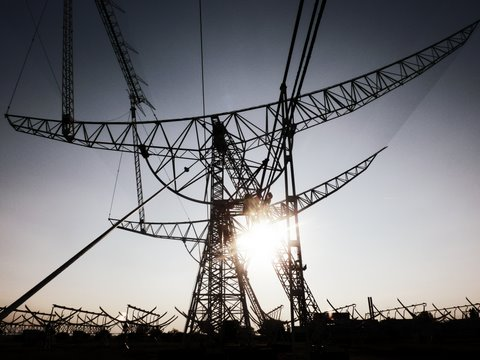
\includegraphics{medicina.jpg}
\caption{The Northern Cross, Medicina, Italy. Photo by G. Foster.}\end{figure}


\chapter{The FITS IDI convention}
\label{index:the-fits-idi-convention}
The FITS Interferometry Data Interchange Convention (“FITS-IDI”) is a set of conventions layered upon the standard FITS format to assist in the interchange of data recorded by interferometric telescopes, particularly at radio frequencies and very long baselines.

FITS IDI is a registered convention in the NASA/IAU FITS working group registry, meaning it is defined and documented to ``a minimum level of completeness and clarity''. FITS IDI files can be read by AIPS, AIPS++ and CASA (although I have only tested with CASA). They are used by the VLBA (Very Long Baseline Array) and JIVE (Joint Institute for VLBI in Europe), among others.

There are a few alternative formats to FITS IDI, such as \href{http://www.atnf.csiro.au/computing/software/miriad/}{Miriad} FITS files, UVFITS files, and \href{http://casa.nrao.edu/docs/userman/UserManse6.html}{Measurement Sets} (MS). Miriad is getting a little long in the tooth, UVFITS is not very well documented, and Measurement Sets are a bit of a pain to create -- plus, a MS isn't a FITS file, so it can't be read by FITS readers.

Much more info on the FITS IDI convention can be found on its \href{http://fits.gsfc.nasa.gov/registry/fitsidi.html}{official page}. If you're not familiar with FITS files, you might also want to look at the actual \href{http://www.aanda.org/index.php?option=com\_article\&access=doi\&doi=10.1051/0004-6361/201015362\&Itemid=129}{FITS definition}. Finally, there are useful FITS resources at the \href{http://fits.gsfc.nasa.gov/fits\_home.html}{NASA FITS website}.


\chapter{Prerequisites}
\label{index:prerequisites}
The actual reading/writing of FITS files is done by the \href{http://www.stsci.edu/resources/software\_hardware/pyfits}{PyFITS} package. You'll also need \href{http://numpy.scipy.org/}{numpy} for array handling and \href{http://lxml.de/}{lxml} for parsing config XML files.

In the file createMedicinaFITS.py, we make use of \href{http://rhodesmill.org/pyephem/}{pyEphem} for astronomical calculations, and \href{http://www.pytables.org/moin}{pyTables} for HDF5 file I/O. Yo


\chapter{Example Usage}
\label{index:example-usage}
A simple example of how to use pyFitsidi.py can be found in the createFitsIDI.py:

\begin{Verbatim}[commandchars=\\\{\}]
\PYG{g+gp}{\textgreater{}\textgreater{}\textgreater{} }\PYG{l+s+sd}{"""}
\PYG{g+gp}{... }\PYG{l+s+sd}{createFitsIDI.py}
\PYG{g+gp}{... }\PYG{l+s+sd}{=============}
\PYG{g+gp}{...}
\PYG{g+gp}{... }\PYG{l+s+sd}{Creates a basic FITS IDI file, with headers created from an XML configuration file.}
\PYG{g+gp}{...}
\PYG{g+gp}{... }\PYG{l+s+sd}{Created by Danny Price on 2011-04-20.}
\PYG{g+gp}{... }\PYG{l+s+sd}{Copyright (c) 2011 The University of Oxford. All rights reserved.}
\PYG{g+gp}{...}
\PYG{g+gp}{... }\PYG{l+s+sd}{"""}
\PYG{g+gp}{...}
\PYG{g+gp}{... }\PYG{c}{\PYGZsh{} Required modules}
\PYG{g+gp}{... }\PYG{k+kn}{import} \PYG{n+nn}{sys}\PYG{o}{,} \PYG{n+nn}{os}
\PYG{g+gp}{... }\PYG{k+kn}{import} \PYG{n+nn}{pyfits} \PYG{k+kn}{as} \PYG{n+nn}{pf}\PYG{o}{,} \PYG{n+nn}{numpy} \PYG{k+kn}{as} \PYG{n+nn}{np}
\PYG{g+gp}{...}
\PYG{g+gp}{... }\PYG{c}{\PYGZsh{} import modules from this package}
\PYG{g+gp}{... }\PYG{k+kn}{from} \PYG{n+nn}{pyFitsidi} \PYG{k+kn}{import} \PYG{o}{*}
\PYG{g+gp}{...}
\PYG{g+gp}{... }\PYG{k}{def} \PYG{n+nf}{main}\PYG{p}{(}\PYG{p}{)}\PYG{p}{:}
\PYG{g+gp}{... }  \PYG{l+s+sd}{"""}
\PYG{g+gp}{... }\PYG{l+s+sd}{  Generate a blank FITS IDI file.}
\PYG{g+gp}{... }\PYG{l+s+sd}{  """}
\PYG{g+gp}{...}
\PYG{g+gp}{... }  \PYG{c}{\PYGZsh{} What are the filenames for our datasets?}
\PYG{g+gp}{... }  \PYG{n}{fitsfile} \PYG{o}{=} \PYG{l+s}{'}\PYG{l+s}{blank.fits}\PYG{l+s}{'}
\PYG{g+gp}{... }  \PYG{n}{config}   \PYG{o}{=} \PYG{l+s}{'}\PYG{l+s}{config/config.xml}\PYG{l+s}{'}
\PYG{g+gp}{...}
\PYG{g+gp}{... }  \PYG{c}{\PYGZsh{} Make a new blank FITS HDU}
\PYG{g+gp}{... }  \PYG{k}{print}\PYG{p}{(}\PYG{l+s}{'}\PYG{l+s}{Creating Primary HDU}\PYG{l+s}{'}\PYG{p}{)}
\PYG{g+gp}{... }  \PYG{k}{print}\PYG{p}{(}\PYG{l+s}{'}\PYG{l+s}{------------------------------------}\PYG{l+s+se}{\PYGZbs{}n}\PYG{l+s}{'}\PYG{p}{)}
\PYG{g+gp}{... }  \PYG{n}{hdu} \PYG{o}{=} \PYG{n}{make\PYGZus{}primary}\PYG{p}{(}\PYG{n}{config}\PYG{p}{)}
\PYG{g+gp}{... }  \PYG{k}{print} \PYG{n}{hdu}\PYG{o}{.}\PYG{n}{header}\PYG{o}{.}\PYG{n}{ascardlist}\PYG{p}{(}\PYG{p}{)}
\PYG{g+gp}{...}
\PYG{g+gp}{... }  \PYG{c}{\PYGZsh{} Go through and generate required tables}
\PYG{g+gp}{... }  \PYG{k}{print}\PYG{p}{(}\PYG{l+s}{'}\PYG{l+s+se}{\PYGZbs{}n}\PYG{l+s}{Creating ARRAY\PYGZus{}GEOMETRY}\PYG{l+s}{'}\PYG{p}{)}
\PYG{g+gp}{... }  \PYG{k}{print}\PYG{p}{(}\PYG{l+s}{'}\PYG{l+s}{------------------------------------}\PYG{l+s}{'}\PYG{p}{)}
\PYG{g+gp}{... }  \PYG{n}{tbl\PYGZus{}array\PYGZus{}geometry} \PYG{o}{=} \PYG{n}{make\PYGZus{}array\PYGZus{}geometry}\PYG{p}{(}\PYG{n}{config}\PYG{o}{=}\PYG{n}{config}\PYG{p}{,} \PYG{n}{num\PYGZus{}rows}\PYG{o}{=}\PYG{l+m+mi}{32}\PYG{p}{)}
\PYG{g+gp}{... }  \PYG{k}{print} \PYG{n}{tbl\PYGZus{}array\PYGZus{}geometry}\PYG{o}{.}\PYG{n}{header}\PYG{o}{.}\PYG{n}{ascardlist}\PYG{p}{(}\PYG{p}{)}
\PYG{g+gp}{...}
\PYG{g+gp}{... }  \PYG{k}{print}\PYG{p}{(}\PYG{l+s}{'}\PYG{l+s+se}{\PYGZbs{}n}\PYG{l+s}{Creating FREQUENCY}\PYG{l+s}{'}\PYG{p}{)}
\PYG{g+gp}{... }  \PYG{k}{print}\PYG{p}{(}\PYG{l+s}{'}\PYG{l+s}{------------------------------------}\PYG{l+s}{'}\PYG{p}{)}
\PYG{g+gp}{... }  \PYG{n}{tbl\PYGZus{}frequency} \PYG{o}{=} \PYG{n}{make\PYGZus{}frequency}\PYG{p}{(}\PYG{n}{config}\PYG{o}{=}\PYG{n}{config}\PYG{p}{,} \PYG{n}{num\PYGZus{}rows}\PYG{o}{=}\PYG{l+m+mi}{1}\PYG{p}{)}
\PYG{g+gp}{... }  \PYG{k}{print} \PYG{n}{tbl\PYGZus{}frequency}\PYG{o}{.}\PYG{n}{header}\PYG{o}{.}\PYG{n}{ascardlist}\PYG{p}{(}\PYG{p}{)}
\PYG{g+gp}{...}
\PYG{g+gp}{... }  \PYG{k}{print}\PYG{p}{(}\PYG{l+s}{'}\PYG{l+s+se}{\PYGZbs{}n}\PYG{l+s}{Creating SOURCE}\PYG{l+s}{'}\PYG{p}{)}
\PYG{g+gp}{... }  \PYG{k}{print}\PYG{p}{(}\PYG{l+s}{'}\PYG{l+s}{------------------------------------}\PYG{l+s}{'}\PYG{p}{)}
\PYG{g+gp}{... }  \PYG{n}{tbl\PYGZus{}source} \PYG{o}{=} \PYG{n}{make\PYGZus{}source}\PYG{p}{(}\PYG{n}{config}\PYG{o}{=}\PYG{n}{config}\PYG{p}{,} \PYG{n}{num\PYGZus{}rows}\PYG{o}{=}\PYG{l+m+mi}{1}\PYG{p}{)}
\PYG{g+gp}{... }  \PYG{k}{print} \PYG{n}{tbl\PYGZus{}source}\PYG{o}{.}\PYG{n}{header}\PYG{o}{.}\PYG{n}{ascardlist}\PYG{p}{(}\PYG{p}{)}
\PYG{g+gp}{...}
\PYG{g+gp}{... }  \PYG{k}{print}\PYG{p}{(}\PYG{l+s}{'}\PYG{l+s+se}{\PYGZbs{}n}\PYG{l+s}{Creating ANTENNA}\PYG{l+s}{'}\PYG{p}{)}
\PYG{g+gp}{... }  \PYG{k}{print}\PYG{p}{(}\PYG{l+s}{'}\PYG{l+s}{------------------------------------}\PYG{l+s}{'}\PYG{p}{)}
\PYG{g+gp}{... }  \PYG{n}{tbl\PYGZus{}antenna} \PYG{o}{=} \PYG{n}{make\PYGZus{}antenna}\PYG{p}{(}\PYG{n}{config}\PYG{o}{=}\PYG{n}{config}\PYG{p}{,} \PYG{n}{num\PYGZus{}rows}\PYG{o}{=}\PYG{l+m+mi}{32}\PYG{p}{)}
\PYG{g+gp}{... }  \PYG{k}{print} \PYG{n}{tbl\PYGZus{}antenna}\PYG{o}{.}\PYG{n}{header}\PYG{o}{.}\PYG{n}{ascardlist}\PYG{p}{(}\PYG{p}{)}
\PYG{g+gp}{...}
\PYG{g+gp}{... }  \PYG{k}{print}\PYG{p}{(}\PYG{l+s}{'}\PYG{l+s+se}{\PYGZbs{}n}\PYG{l+s}{Creating UV\PYGZus{}DATA}\PYG{l+s}{'}\PYG{p}{)}
\PYG{g+gp}{... }  \PYG{k}{print}\PYG{p}{(}\PYG{l+s}{'}\PYG{l+s}{------------------------------------}\PYG{l+s}{'}\PYG{p}{)}
\PYG{g+gp}{... }  \PYG{c}{\PYGZsh{} Number of rows req. depends on num. time dumps and num. of baselines}
\PYG{g+gp}{... }  \PYG{c}{\PYGZsh{} Once you have data, it would be worth setting these dimensions automatically}
\PYG{g+gp}{... }  \PYG{c}{\PYGZsh{} For now, we're hard-wiring in 1 time dump, 528 baselines (32 element array)}
\PYG{g+gp}{... }  \PYG{p}{(}\PYG{n}{t\PYGZus{}len}\PYG{p}{,} \PYG{n}{bl\PYGZus{}len}\PYG{p}{)} \PYG{o}{=} \PYG{p}{(}\PYG{l+m+mi}{1}\PYG{p}{,}\PYG{l+m+mi}{528}\PYG{p}{)}
\PYG{g+gp}{... }  \PYG{n}{tbl\PYGZus{}uv\PYGZus{}data} \PYG{o}{=} \PYG{n}{make\PYGZus{}uv\PYGZus{}data}\PYG{p}{(}\PYG{n}{config}\PYG{o}{=}\PYG{n}{config}\PYG{p}{,} \PYG{n}{num\PYGZus{}rows}\PYG{o}{=}\PYG{n}{t\PYGZus{}len}\PYG{o}{*}\PYG{n}{bl\PYGZus{}len}\PYG{p}{)}
\PYG{g+gp}{... }  \PYG{k}{print} \PYG{n}{tbl\PYGZus{}antenna}\PYG{o}{.}\PYG{n}{header}\PYG{o}{.}\PYG{n}{ascardlist}\PYG{p}{(}\PYG{p}{)}
\PYG{g+gp}{...}
\PYG{g+gp}{... }  \PYG{k}{print}\PYG{p}{(}\PYG{l+s}{'}\PYG{l+s+se}{\PYGZbs{}n}\PYG{l+s}{Creating HDU list}\PYG{l+s}{'}\PYG{p}{)}
\PYG{g+gp}{... }  \PYG{k}{print}\PYG{p}{(}\PYG{l+s}{'}\PYG{l+s}{------------------------------------}\PYG{l+s}{'}\PYG{p}{)}
\PYG{g+gp}{... }  \PYG{n}{hdulist} \PYG{o}{=} \PYG{n}{pf}\PYG{o}{.}\PYG{n}{HDUList}\PYG{p}{(}
\PYG{g+gp}{... }              \PYG{p}{[}\PYG{n}{hdu}\PYG{p}{,}
\PYG{g+gp}{... }              \PYG{n}{tbl\PYGZus{}array\PYGZus{}geometry}\PYG{p}{,}
\PYG{g+gp}{... }              \PYG{n}{tbl\PYGZus{}frequency}\PYG{p}{,}
\PYG{g+gp}{... }              \PYG{n}{tbl\PYGZus{}antenna}\PYG{p}{,}
\PYG{g+gp}{... }              \PYG{n}{tbl\PYGZus{}source}\PYG{p}{,}
\PYG{g+gp}{... }              \PYG{n}{tbl\PYGZus{}uv\PYGZus{}data}
\PYG{g+gp}{... }              \PYG{p}{]}\PYG{p}{)}
\PYG{g+gp}{...}
\PYG{g+gp}{... }  \PYG{k}{print}\PYG{p}{(}\PYG{l+s}{'}\PYG{l+s+se}{\PYGZbs{}n}\PYG{l+s}{Verifying integrity...}\PYG{l+s}{'}\PYG{p}{)}
\PYG{g+gp}{... }  \PYG{n}{hdulist}\PYG{o}{.}\PYG{n}{verify}\PYG{p}{(}\PYG{p}{)}
\PYG{g+gp}{...}
\PYG{g+gp}{... }  \PYG{k}{if}\PYG{p}{(}\PYG{n}{os}\PYG{o}{.}\PYG{n}{path}\PYG{o}{.}\PYG{n}{isfile}\PYG{p}{(}\PYG{n}{fitsfile}\PYG{p}{)}\PYG{p}{)}\PYG{p}{:}
\PYG{g+gp}{... }    \PYG{k}{print}\PYG{p}{(}\PYG{l+s}{'}\PYG{l+s}{Removing existing file }\PYG{l+s+si}{\PYGZpc{}s}\PYG{l+s}{...}\PYG{l+s}{'}\PYG{p}{)}\PYG{o}{\PYGZpc{}}\PYG{n}{fitsfile}
\PYG{g+gp}{... }    \PYG{n}{os}\PYG{o}{.}\PYG{n}{remove}\PYG{p}{(}\PYG{n}{fitsfile}\PYG{p}{)}
\PYG{g+gp}{... }  \PYG{k}{print}\PYG{p}{(}\PYG{l+s}{'}\PYG{l+s}{Writing to file }\PYG{l+s+si}{\PYGZpc{}s}\PYG{l+s}{...}\PYG{l+s}{'}\PYG{p}{)}\PYG{o}{\PYGZpc{}}\PYG{n}{fitsfile}
\PYG{g+gp}{... }  \PYG{n}{hdulist}\PYG{o}{.}\PYG{n}{writeto}\PYG{p}{(}\PYG{n}{fitsfile}\PYG{p}{)}
\PYG{g+gp}{...}
\PYG{g+gp}{... }  \PYG{k}{print}\PYG{p}{(}\PYG{l+s}{'}\PYG{l+s}{Done.}\PYG{l+s}{'}\PYG{p}{)}
\PYG{g+gp}{...}
\PYG{g+gp}{...}
\PYG{g+gp}{... }\PYG{k}{if} \PYG{n}{\PYGZus{}\PYGZus{}name\PYGZus{}\PYGZus{}} \PYG{o}{==} \PYG{l+s}{'}\PYG{l+s}{\PYGZus{}\PYGZus{}main\PYGZus{}\PYGZus{}}\PYG{l+s}{'}\PYG{p}{:}
\PYG{g+gp}{... }  \PYG{n}{main}\PYG{p}{(}\PYG{p}{)}
\end{Verbatim}

A more complicated example is shown in createMedicinaFITS.py. In this file, a complete FITS IDI file is generated from an XML config file and a HDF5 data file. While the XML and HDF5 data are specific to the Medicina BEST-2 telescope, this file could be adapted as required.

In createMedicinaFITS.py, only the mandatory binary tables are created: array\_geometry, antenna, frequency, source and uv\_data.


\chapter{Module Documentation}
\label{index:module-pyFitsidi}\label{index:module-documentation}
\index{pyFitsidi (module)}

\section{pyFitsidi.py}
\label{index:pyfitsidi-py}
Created by Danny Price on 2011-04-28.
Copyright (c) 2011 The University of Oxford. All rights reserved.

This file is a collection of modules for creating blank FITS IDI files.
It consists mainly of pretty basic functions to create blank tables.

The FITS handling is all done by pyFits, and blank arrays are created
with numpy. So you'll need to have both of these installed on your machine.
In addition, the config xml file is read with lxml, so install that too.


\subsection{FITS-IDI Table Overview}
\label{index:fits-idi-table-overview}
Here is a quick rundown of the tables that this script can make.
Not all these tables are mandatory, so I've starred the ones which are the most
important to understand and to get into your dataset.
\begin{itemize}
\item {} 
\textbf{ANTENNA}           Antenna polarization information

\item {} 
\textbf{ARRAY\_GEOMETRY}    Time system information and antenna coordinates

\item {} 
FLAG                  Flagged data

\item {} 
\textbf{FREQUENCY}         Frequency setups

\item {} 
GAIN\_CURVE            Antenna gain curves

\item {} 
INTERFEROMETER\_MODEL  Correlator model

\item {} 
PHASE-CAL             Phase cal measurements

\item {} 
\textbf{SOURCE}            Sources observed

\item {} 
SYSTEM\_TEMPERATURE    System and antenna temperatures

\item {} 
\textbf{UV\_DATA}           Visibility data

\end{itemize}

These tables are new from the FITS IDI update, and are all optional:
\begin{itemize}
\item {} 
BANDPASS              Bandpass functions

\item {} 
BASELINE              Baseline-specific gain factors

\item {} 
CALIBRATION           Gains as a function of time

\item {} 
WEATHER               Meteorological data

\end{itemize}


\subsection{Module listing}
\label{index:module-listing}
\index{make\_antenna() (in module pyFitsidi)}

\begin{fulllineitems}
\phantomsection\label{index:pyFitsidi.make_antenna}\pysiglinewithargsret{\code{pyFitsidi.}\bfcode{make\_antenna}}{\emph{config='config.xml'}, \emph{num\_rows=1}}{}
Creates a vanilla ANTENNA table HDU
\begin{quote}\begin{description}
\item[{Parameters }] \leavevmode
\textbf{config: string} :
\begin{quote}

filename of xml configuration file, defaults to `config,xml'
\end{quote}

\textbf{num\_rows: int} :
\begin{quote}

number of rows to generate. Rows will be filled with numpy zeros.
\end{quote}

\end{description}\end{quote}
\paragraph{Notes}

CASA didn't like importing POLCALA and POLCALB, so they are currently commented out.

Table is built with the following columns:
\begin{itemize}
\item {} 
TIME: Difference of antenna table time interval centre time and RDATE 0 hours

\item {} 
TIME\_INTERVAL: Antenna table time interval width

\item {} 
ANNAME: Antenna name, should match value in ARRAY\_GEOMETRY

\item {} 
ANTENNA\_NO: Antemma ID number for station

\item {} 
ARRAY:    Array ID number

\item {} 
FREQID:   Frequency setup ID number

\item {} 
NO\_LEVELS:Number of digitiser levels

\item {} 
POLYTYA:  Feed A polarisation direction

\item {} 
POLAA:    Feed A polarisation (degrees)

\item {} 
POLCALA:  Feed A polarisation parameters

\item {} 
POLYTYB:  As above, for feed B

\item {} 
POLAB:    As above, for feed B

\item {} 
POLCALB:  As above, for feed B

\end{itemize}

\end{fulllineitems}


\index{make\_array\_geometry() (in module pyFitsidi)}

\begin{fulllineitems}
\phantomsection\label{index:pyFitsidi.make_array_geometry}\pysiglinewithargsret{\code{pyFitsidi.}\bfcode{make\_array\_geometry}}{\emph{config='config.xml'}, \emph{num\_rows=1}}{}
Creates a vanilla ARRAY\_GEOMETRY table HDU.

One row is required for each antenna in the array (num\_rows)
\begin{quote}\begin{description}
\item[{Parameters }] \leavevmode
\textbf{config: string} :
\begin{quote}

filename of xml configuration file, defaults to `config,xml'
\end{quote}

\textbf{num\_rows: int} :
\begin{quote}

number of rows to generate. Rows will be filled with numpy zeros.
\end{quote}

\end{description}\end{quote}
\paragraph{Notes}

Table is built with the following columns:
\begin{itemize}
\item {} 
ANNAME: Antenna name

\item {} 
STABXYZ: Antenna relative position vector ECI components, in meters

\item {} 
DERXYZ: Antenna velocity vector components, in meters/sec

\item {} 
ORBPARM: Orbital parameters

\item {} 
NOSTA: Antenna ID number for station

\item {} 
MNTSTA: Antenna mount type (0 is alt-azimuth)

\item {} 
STAXOF: Antenna axis offset, in meters

\item {} 
DIAMETER: Antenna diameter (optional)

\end{itemize}

\end{fulllineitems}


\index{make\_bandpass() (in module pyFitsidi)}

\begin{fulllineitems}
\phantomsection\label{index:pyFitsidi.make_bandpass}\pysiglinewithargsret{\code{pyFitsidi.}\bfcode{make\_bandpass}}{\emph{config='config.xml'}, \emph{num\_rows=1}}{}
Creates a vanilla BANDPASS table HDU
\begin{quote}\begin{description}
\item[{Parameters }] \leavevmode
\textbf{config: string} :
\begin{quote}

filename of xml configuration file, defaults to `config,xml'
\end{quote}

\textbf{num\_rows: int} :
\begin{quote}

number of rows to generate. Rows will be filled with numpy zeros.
\end{quote}

\end{description}\end{quote}
\paragraph{Notes}

Table is built with the following columns:
\begin{itemize}
\item {} 
TIME: Difference of bandpass table time int center time and RDATE 0 hours

\item {} 
TIME\_INTERVAL: Bandpass table time interval width

\item {} 
SOURCE\_ID:  Source ID number

\item {} 
ANTENNA\_NO: Antenna ID number for station

\item {} 
ARRAY:      Array ID number

\item {} 
FREQID:     Frequency setup ID number (should match ANTENNA)

\item {} 
BANDWIDTH:  Frequency band width described by bandpass

\item {} 
BAND\_FREQ:  Frequency band base offset

\item {} 
REFANT\_1:   Reference antenna ID number

\item {} 
BREAL\_1:    Bandpass response real componet

\item {} 
BIMAG\_1:    Bandpass response imaginary component

\end{itemize}

\end{fulllineitems}


\index{make\_flag() (in module pyFitsidi)}

\begin{fulllineitems}
\phantomsection\label{index:pyFitsidi.make_flag}\pysiglinewithargsret{\code{pyFitsidi.}\bfcode{make\_flag}}{\emph{config='config.xml'}, \emph{num\_rows=1}}{}
Creates a vanilla FLAG table HDU
\begin{quote}\begin{description}
\item[{Parameters }] \leavevmode
\textbf{config: string} :
\begin{quote}

filename of xml configuration file, defaults to `config,xml'
\end{quote}

\textbf{num\_rows: int} :
\begin{quote}

number of rows to generate. Rows will be filled with numpy zeros.
\end{quote}

\end{description}\end{quote}
\paragraph{Notes}

This table is optional.

Table is built with the following columns:
\begin{itemize}
\item {} 
SOURCE\_ID Source ID number

\item {} 
ARRAY     Array number

\item {} 
ANTS      Antenna numbers

\item {} 
FREQID    Frequency setup number

\item {} 
TIMERANG  Time range

\item {} 
BANDS     Band flags

\item {} 
CHANS     Channel range

\item {} 
PFLAGS    Polarization flags

\item {} 
REASON    Reason for flag

\item {} 
SEVERITY  Severity code

\end{itemize}

\end{fulllineitems}


\index{make\_frequency() (in module pyFitsidi)}

\begin{fulllineitems}
\phantomsection\label{index:pyFitsidi.make_frequency}\pysiglinewithargsret{\code{pyFitsidi.}\bfcode{make\_frequency}}{\emph{config='config.xml'}, \emph{num\_rows=1}}{}
Creates a vanilla FREQUENCY table HDU
\begin{quote}\begin{description}
\item[{Parameters }] \leavevmode
\textbf{config: string} :
\begin{quote}

filename of xml configuration file, defaults to `config,xml'
\end{quote}

\textbf{num\_rows: int} :
\begin{quote}

number of rows to generate. Rows will be filled with numpy zeros.
\end{quote}

\end{description}\end{quote}
\paragraph{Notes}

Table is built with the following columns:
\begin{itemize}
\item {} 
FREQID:   Frequency setup ID number

\item {} 
BANDFREQ: Frequency band base offset (Hz)

\item {} 
CH\_WIDTH: Frequency channel width (Hz)

\item {} 
TOTAL\_BANDWIDTH: Frequency bandwidth (Hz)

\item {} 
SIDEBAND: Sideband flag (1 indicates upper sideband)

\item {} 
BB\_CHAN:  ?

\end{itemize}

\end{fulllineitems}


\index{make\_gain\_curve() (in module pyFitsidi)}

\begin{fulllineitems}
\phantomsection\label{index:pyFitsidi.make_gain_curve}\pysiglinewithargsret{\code{pyFitsidi.}\bfcode{make\_gain\_curve}}{\emph{config='config.xml'}, \emph{num\_rows=1}}{}
Creates a vanilla GAIN\_CURVE table HDU
\begin{quote}\begin{description}
\item[{Parameters }] \leavevmode
\textbf{config: string} :
\begin{quote}

filename of xml configuration file, defaults to `config,xml'
\end{quote}

\textbf{num\_rows: int} :
\begin{quote}

number of rows to generate. Rows will be filled with numpy zeros.
\end{quote}

\end{description}\end{quote}
\paragraph{Notes}

This is an optional table (we will not include it). 
Todo: Add switch to allow dual polarisation.

Table is built with the following columns:
\begin{itemize}
\item {} 
ANTENNA\_NO  Antenna number

\item {} 
ARRAY       Array number

\item {} 
FREQID      Frequency setup number

\item {} 
TYPE\_1      Gain curve types for polarization 1

\item {} 
NTERM\_1     Numbers of terms or entries for polarization 1

\item {} 
X\_TYP\_1     x value types for polarization 1

\item {} 
Y\_TYP\_1     y value types for polarization 1

\item {} 
X\_VAL\_1     x values for polarization 1

\item {} 
Y\_VAL\_1     y values for polarization 1

\item {} 
GAIN\_1      Relative gain values for polarization 1

\item {} 
SENS\_1      Sensitivities for polarization 1

\end{itemize}

\end{fulllineitems}


\index{make\_interferometer\_model() (in module pyFitsidi)}

\begin{fulllineitems}
\phantomsection\label{index:pyFitsidi.make_interferometer_model}\pysiglinewithargsret{\code{pyFitsidi.}\bfcode{make\_interferometer\_model}}{\emph{config='config.xml'}, \emph{num\_rows=1}}{}
Creates a vanilla INTERFEROMETER\_MODEL table HDU.
\begin{quote}\begin{description}
\item[{Parameters }] \leavevmode
\textbf{config: string} :
\begin{quote}

filename of xml configuration file, defaults to `config,xml'
\end{quote}

\textbf{num\_rows: int} :
\begin{quote}

number of rows to generate. Rows will be filled with numpy zeros.
\end{quote}

\end{description}\end{quote}
\paragraph{Notes}

This table is optional, and is not included in Medicina FITS IDI

Table is built with the following columns:
\begin{itemize}
\item {} 
TIME          Starting time of interval

\item {} 
TIME\_INTERVAL Duration of interval

\item {} 
SOURCE\_ID     Source ID number

\item {} 
ANTENNA\_NO    Antenna number

\item {} 
ARRAY         Array number

\item {} 
FREQID        Frequency setup number

\item {} 
I.FAR.ROT     Ionospheric Faraday rotation

\item {} 
FREQ\_VAR      Time-variable frequency offsets

\item {} 
PDELAY\_1      Phase delay polynomials for polarization 1

\item {} 
GDELAY\_1      Group delay polynomials for polarization 1

\item {} 
PRATE\_1       Phase delay rate polynomials for polarization 1

\item {} 
GRATE\_1       Group rate polynomials for polarization 1

\item {} 
DISP\_1        Dispersive delay for polarization 1 at 1m wavelength

\item {} 
DDISP\_1       Rate of change of dispersive del for pol 1 at 1m

\end{itemize}

\end{fulllineitems}


\index{make\_phase\_cal() (in module pyFitsidi)}

\begin{fulllineitems}
\phantomsection\label{index:pyFitsidi.make_phase_cal}\pysiglinewithargsret{\code{pyFitsidi.}\bfcode{make\_phase\_cal}}{\emph{config='config.xml'}, \emph{num\_rows=1}}{}
Creates a vanilla PHASE-CAL table HDU
\begin{quote}\begin{description}
\item[{Parameters }] \leavevmode
\textbf{config: string} :
\begin{quote}

filename of xml configuration file, defaults to `config,xml'
\end{quote}

\textbf{num\_rows: int} :
\begin{quote}

number of rows to generate. Rows will be filled with numpy zeros.
\end{quote}

\end{description}\end{quote}
\paragraph{Notes}

This is an optional table (we will not include it)

Table is built with the following columns:
\begin{itemize}
\item {} 
TIME          Central time of interval covered

\item {} 
TIME\_INTERVAL Duration of interval

\item {} 
SOURCE\_ID     Source ID number

\item {} 
ANTENNA\_NO    Antenna number

\item {} 
ARRAY         Array number

\item {} 
FREQID        Frequency setup number

\item {} 
CABLE\_CAL     Cable calibration measurement

\item {} 
STATE\_1       State counts for polarization 1

\item {} 
PC\_FREQ\_1     Phase cal tone frequencies for polarization 1

\item {} 
PC\_REAL\_1     real parts of phase-cal measurements for pol 1

\item {} 
PC\_IMAG\_1     imaginary parts of phasecal measurements for pol 1

\item {} 
PC\_RATE\_1     phase-cal rates for polarization 1

\end{itemize}

\end{fulllineitems}


\index{make\_primary() (in module pyFitsidi)}

\begin{fulllineitems}
\phantomsection\label{index:pyFitsidi.make_primary}\pysiglinewithargsret{\code{pyFitsidi.}\bfcode{make\_primary}}{\emph{config='config.xml'}}{}
Creates the primary header data unit (HDU).

This function generates header keywords from the file headers/primary.tpl
\begin{quote}\begin{description}
\item[{Parameters }] \leavevmode
\textbf{config: string} :
\begin{quote}

filename of xml configuration file, defaults to `config,xml'
\end{quote}

\end{description}\end{quote}

\end{fulllineitems}


\index{make\_source() (in module pyFitsidi)}

\begin{fulllineitems}
\phantomsection\label{index:pyFitsidi.make_source}\pysiglinewithargsret{\code{pyFitsidi.}\bfcode{make\_source}}{\emph{config='config.xml'}, \emph{num\_rows=1}}{}
Creates a vanilla SOURCE table HDU
\begin{quote}\begin{description}
\item[{Parameters }] \leavevmode
\textbf{config: string} :
\begin{quote}

filename of xml configuration file, defaults to `config,xml'
\end{quote}

\textbf{num\_rows: int} :
\begin{quote}

number of rows to generate. Rows will be filled with numpy zeros.
\end{quote}

\end{description}\end{quote}
\paragraph{Notes}

Table is built with the following columns:
\begin{itemize}
\item {} 
SOURCE\_ID Source ID number

\item {} 
SOURCE    Source name

\item {} 
QUAL      Source qualifier number.

\item {} 
CALCODE   Source calibrator code.

\item {} 
FREQID    Source frequency ID

\item {} 
IFLUX     Source I flux density

\item {} 
QFLUX     Source Q flux density

\item {} 
UFLUX     Source U flux density

\item {} 
VFLUX     SourceV flux density

\item {} 
ALPHA     Source spectral index

\item {} 
FREQOFF   Source frequency offset

\item {} 
RAEPO     Source J2000 equatorial position RA coordinate

\item {} 
DECPO     Source J2000 equatorial position DEC coordinate

\item {} 
EQUINOX   Mean Equinox

\item {} 
RAAPP     Source apparent equatorial position RA coordinate

\item {} 
DECAPP    Source apparent equatorial position DEC coordinate

\item {} 
SYSVEL    Systematic velocity.

\item {} 
VELTYP    Systematic velocity reference frame.

\item {} 
VELDEF    Systematic velocity convention.

\item {} 
RESTFREQ  Line rest frequency.

\item {} 
PMRA      Source proper motion RA coordinate

\item {} 
PMDEC     Source proper motion DEC coordinate

\item {} 
PARALLAX  Source parallax.

\end{itemize}

\end{fulllineitems}


\index{make\_system\_temperature() (in module pyFitsidi)}

\begin{fulllineitems}
\phantomsection\label{index:pyFitsidi.make_system_temperature}\pysiglinewithargsret{\code{pyFitsidi.}\bfcode{make\_system\_temperature}}{\emph{config='config.xml'}, \emph{num\_rows=1}}{}
Creates a vanilla SYSTEM\_TEMPERATURE table HDU
\begin{quote}\begin{description}
\item[{Parameters }] \leavevmode
\textbf{config: string} :
\begin{quote}

filename of xml configuration file, defaults to `config,xml'
\end{quote}

\textbf{num\_rows: int} :
\begin{quote}

number of rows to generate. Rows will be filled with numpy zeros.
\end{quote}

\end{description}\end{quote}
\paragraph{Notes}

This is an optional table.
Todo: add dual pol support.

Table is built with the following columns:
\begin{itemize}
\item {} 
TIME          Central time of interval covered

\item {} 
TIME\_INTERVAL Duration of interval

\item {} 
SOURCE\_ID     Source ID number

\item {} 
ANTENNA\_NO    Antenna number

\item {} 
ARRAY         Array number

\item {} 
FREQID        Frequency setup number

\item {} 
TSYS\_1        System temperatures for polarization 1

\item {} 
TANT\_1        Antenna temperatures for polarization 1

\end{itemize}

\end{fulllineitems}


\index{make\_uv\_data() (in module pyFitsidi)}

\begin{fulllineitems}
\phantomsection\label{index:pyFitsidi.make_uv_data}\pysiglinewithargsret{\code{pyFitsidi.}\bfcode{make\_uv\_data}}{\emph{config='config.xml'}, \emph{num\_rows=1}}{}
Creates a vanilla UV\_DATA table HDU
\begin{quote}\begin{description}
\item[{Parameters }] \leavevmode
\textbf{config: string} :
\begin{quote}

filename of xml configuration file, defaults to `config,xml'
\end{quote}

\textbf{num\_rows: int} :
\begin{quote}

number of rows to generate. Rows will be filled with numpy zeros.
\end{quote}

\end{description}\end{quote}
\paragraph{Notes}

Table is built with the following columns:
\begin{itemize}
\item {} 
UU           Baseline vector U coordinate (seconds)

\item {} 
VV           Baseline vector V coordinate

\item {} 
WW           Baseline vector W coordinate

\item {} 
DATE         UTC Julian day value for time 00:00:00  on the day of the observation

\item {} 
TIME         Fraction of Julian day from midnight to timestamp on day of observation.

\item {} 
BASELINE     Antenna baseline pair ID.

\item {} 
FILTER       VLBA filter ID

\item {} 
SOURCE       Data source ID

\item {} 
FREQID       Data frequency setup ID

\item {} 
INTTIM       Data integration time

\item {} 
WEIGHT       Data weights (one element for each freq channel)

\item {} 
GATEID       VLBA gate ID

\item {} 
FLUX         UV visibility data matrix

\end{itemize}

\end{fulllineitems}


\index{parseConfig() (in module pyFitsidi)}

\begin{fulllineitems}
\phantomsection\label{index:pyFitsidi.parseConfig}\pysiglinewithargsret{\code{pyFitsidi.}\bfcode{parseConfig}}{\emph{tagname}, \emph{config='config.xml'}}{}
Finds tagname, in elementTree x, parses and returns dictionary of values
This is a helper function, and is not usually called directly

\end{fulllineitems}

\phantomsection\label{index:module-astroCoords}
\index{astroCoords (module)}

\section{astroCoords.py}
\label{index:astrocoords-py}
Some useful functions for converting in between Right Ascension (hours,mins,secs)
and Declination (degrees,mins,secs) to degrees and radians. These functions are
all named in the same format: a2b(), where a is the original data, and b is the new
data format.

All of this type of basic stuff can be done with pyEphem or similar, but I wanted
something super simple.

Created by Danny Price on 2011-05-01.
Copyright (c) 2011 The University of Oxford. All rights reserved.


\subsection{Module listing}
\label{index:id1}
\index{decdms2deg() (in module astroCoords)}

\begin{fulllineitems}
\phantomsection\label{index:astroCoords.decdms2deg}\pysiglinewithargsret{\code{astroCoords.}\bfcode{decdms2deg}}{\emph{deg}, \emph{min}, \emph{sec}}{}
Converts degrees, minutes seconds into degrees
i.e. a floating point number in range (0,360)
\begin{quote}\begin{description}
\item[{Parameters }] \leavevmode
\textbf{deg: int} :
\begin{quote}

degrees to be converted (from 0 to 360)
\end{quote}

\textbf{min: int} :
\begin{quote}

minutes to be converted (from 0 to 60)
\end{quote}

\textbf{sec: float} :
\begin{quote}

seconds to be converted (from 0.0 to 60.0)
\end{quote}

\end{description}\end{quote}

\end{fulllineitems}


\index{decdms2rad() (in module astroCoords)}

\begin{fulllineitems}
\phantomsection\label{index:astroCoords.decdms2rad}\pysiglinewithargsret{\code{astroCoords.}\bfcode{decdms2rad}}{\emph{deg}, \emph{min}, \emph{sec}}{}
Converts degrees, minutes seconds into radians 
i.e. a floating point number in range (0,2pi)
\begin{quote}\begin{description}
\item[{Parameters }] \leavevmode
\textbf{deg: int} :
\begin{quote}

degrees to be converted (from 0 to 360)
\end{quote}

\textbf{min: int} :
\begin{quote}

minutes to be converted (from 0 to 60)
\end{quote}

\textbf{sec: float} :
\begin{quote}

seconds to be converted (from 0.0 to 60.0)
\end{quote}

\end{description}\end{quote}

\end{fulllineitems}


\index{deg2decdms() (in module astroCoords)}

\begin{fulllineitems}
\phantomsection\label{index:astroCoords.deg2decdms}\pysiglinewithargsret{\code{astroCoords.}\bfcode{deg2decdms}}{\emph{degrees}}{}
Convert number in degrees to declination degs, arcmins, arcsecs
Returns in list (hours,mins,secs)
\begin{quote}\begin{description}
\item[{Parameters }] \leavevmode
\textbf{degrees: float} :
\begin{quote}

degrees to be converted (from 0 to 360)
\end{quote}

\end{description}\end{quote}

\end{fulllineitems}


\index{deg2rad() (in module astroCoords)}

\begin{fulllineitems}
\phantomsection\label{index:astroCoords.deg2rad}\pysiglinewithargsret{\code{astroCoords.}\bfcode{deg2rad}}{\emph{degrees}}{}
Converts from degrees to radians.
This is just a numpy call...
\begin{quote}\begin{description}
\item[{Parameters }] \leavevmode
\textbf{degrees: float} :
\begin{quote}

degrees to be converted (from 0 to 360)
\end{quote}

\end{description}\end{quote}

\end{fulllineitems}


\index{deg2rahms() (in module astroCoords)}

\begin{fulllineitems}
\phantomsection\label{index:astroCoords.deg2rahms}\pysiglinewithargsret{\code{astroCoords.}\bfcode{deg2rahms}}{\emph{degrees}}{}
Convert number in degrees to right ascension HH,MM,SS.SS
Returns in list (hours,mins,secs)
\begin{quote}\begin{description}
\item[{Parameters }] \leavevmode
\textbf{degrees: float} :
\begin{quote}

degrees to be converted (from 0 to 360)
\end{quote}

\end{description}\end{quote}

\end{fulllineitems}


\index{rad2decdms() (in module astroCoords)}

\begin{fulllineitems}
\phantomsection\label{index:astroCoords.rad2decdms}\pysiglinewithargsret{\code{astroCoords.}\bfcode{rad2decdms}}{\emph{radians}}{}
Convert number in radians to declination degs, arcmins, arcsecs
Returns in list (hours,mins,secs)
\begin{quote}\begin{description}
\item[{Parameters }] \leavevmode
\textbf{radians: float} :
\begin{quote}

radians to be converted (from 0 to 2 pi)
\end{quote}

\end{description}\end{quote}

\end{fulllineitems}


\index{rad2deg() (in module astroCoords)}

\begin{fulllineitems}
\phantomsection\label{index:astroCoords.rad2deg}\pysiglinewithargsret{\code{astroCoords.}\bfcode{rad2deg}}{\emph{radians}}{}
Converts from radians to degrees.
This is just a numpy call...
\begin{quote}\begin{description}
\item[{Parameters }] \leavevmode
\textbf{radians: float} :
\begin{quote}

radians to be converted (from 0 to 2 pi)
\end{quote}

\end{description}\end{quote}

\end{fulllineitems}


\index{rad2rahms() (in module astroCoords)}

\begin{fulllineitems}
\phantomsection\label{index:astroCoords.rad2rahms}\pysiglinewithargsret{\code{astroCoords.}\bfcode{rad2rahms}}{\emph{radians}}{}
Convert number in radians to right ascension H,M,SS.SS
Returns tuple (hours,mins,secs)
\begin{quote}\begin{description}
\item[{Parameters }] \leavevmode
\textbf{radians: float} :
\begin{quote}

radians to be converted (from 0 to 2 pi)
\end{quote}

\end{description}\end{quote}

\end{fulllineitems}


\index{rahms2deg() (in module astroCoords)}

\begin{fulllineitems}
\phantomsection\label{index:astroCoords.rahms2deg}\pysiglinewithargsret{\code{astroCoords.}\bfcode{rahms2deg}}{\emph{h}, \emph{m}, \emph{s}}{}
Converts list (hours,minutes,seconds) to degrees
Value returned in range (0,360)
\begin{quote}\begin{description}
\item[{Parameters }] \leavevmode
\textbf{h: int} :
\begin{quote}

hour angle to be converted (from 0 to 24)
\end{quote}

\textbf{h: int} :
\begin{quote}

minutes to be converted (from 0 to 60)
\end{quote}

\textbf{s: float} :
\begin{quote}

seconds to be converted (from 0.0 to 60.0)
\end{quote}

\end{description}\end{quote}

\end{fulllineitems}


\index{rahms2rad() (in module astroCoords)}

\begin{fulllineitems}
\phantomsection\label{index:astroCoords.rahms2rad}\pysiglinewithargsret{\code{astroCoords.}\bfcode{rahms2rad}}{\emph{h}, \emph{m}, \emph{s}}{}
Converts list (hours,minutes,seconds) to radians
Value returned in range (0,2pi)
\begin{quote}\begin{description}
\item[{Parameters }] \leavevmode
\textbf{h: int} :
\begin{quote}

hour angle to be converted (from 0 to 24)
\end{quote}

\textbf{h: int} :
\begin{quote}

minutes to be converted (from 0 to 60)
\end{quote}

\textbf{s: float} :
\begin{quote}

seconds to be converted (from 0.0 to 60.0)
\end{quote}

\end{description}\end{quote}

\end{fulllineitems}



\renewcommand{\indexname}{Python Module Index}
\begin{theindex}
\def\bigletter#1{{\Large\sffamily#1}\nopagebreak\vspace{1mm}}
\bigletter{a}
\item {\texttt{astroCoords}}, \pageref{index:module-astroCoords}
\indexspace
\bigletter{p}
\item {\texttt{pyFitsidi}}, \pageref{index:module-pyFitsidi}
\end{theindex}

\renewcommand{\indexname}{Index}
\printindex
\end{document}
